\chapter{Introducción}

\vspace{-0.5cm}

\begin{flushright}
  \emph{\guillemotleft If we knew what we were doing, it wouldn't be
    called research, would it?\guillemotright}\\ \textbf{Albert Einstein}
\end{flushright}
\hyphenation{Po-pu-larly}
\grayMinitoc

\parindent=16mm

\CAPstart{L}{os}~ \ac{FPGA} son dispositivos de hardware reconfigurables que permiten implementar circuitos digitales personalizados sin necesidad de fabricar un chip desde cero. Están compuestos por una matriz de bloques lógicos programables y una red de interconexiones que puede configurarse para realizar prácticamente cualquier función lógica. En la actualidad, l. Esto desemboca en que todas las fases necesarias en la realización del diseño tienen que estar optimizadas para no sufrir contratiempos inesperados. Esta flexibilidad los convierte en una herramienta fundamental tanto en investigación como en desarrollo industrial, ya que permiten probar y optimizar arquitecturas antes de su producción física, en un mercado cada vez más competitivo, donde las nuevas arquitecturas de \textit{hardware} son lanzadas al mercado anualmente, a veces incluso reduciéndose este valor a la mitad. A diferencia de un microprocesador fijo, un FPGA puede adaptarse a distintos algoritmos, interfaces y arquitecturas, lo que lo hace ideal para prototipado rápido, procesamiento de señales, aplicaciones de alta velocidad y desarrollo de procesadores personalizados como los basados en \ac{RISC-V}. Esta arquitectura ha emergido como una alternativa abierta y flexible frente a arquitecturas propietarias como \ac{ARM}, especialmente en el desarrollo sobre FPGAs. Mientras que ARM ofrece núcleos muy optimizados pero bajo licencia y con limitaciones en la personalización, RISC-V permite a los diseñadores modificar y extender la arquitectura según las necesidades específicas del proyecto. En entornos de FPGA, esta apertura es especialmente valiosa, ya que facilita la experimentación con extensiones personalizadas, la integración con periféricos específicos y la adaptación a aplicaciones concretas. Además, la creciente comunidad y ecosistema de herramientas libres en torno a RISC-V reduce barreras de entrada y fomenta la innovación, donde la experimentación y la optimización del procesador forman parte del objetivo principal. RISC-V es aún una arquitectura en proceso de adaptación a nivel global. A pesar de ello, son muchas las empresas que están realizando la transición hacia esta arquitectura, como la conocida Nvidia \cite{nvidiaRISCV}, anunciando hace un mes que CUDA tendrá soporte a RISC-V. Sin embargo, no son solo las empresas las que participan en su desarrollo: actualmente, hay gran cantidad de proyectos sobre esta arquitectura, como es el simulador de núcleos RISC-V: el proyeto \ac{X-HEEP} \cite{machetti2024xheep} desarrollado por el \ac{EPFL} en Lausanne, Suiza. Será precisamente este simulador el empleado en este \ac{TFM} para realizar validaciones y mediciones de rendimiento sobre el diseño \textit{hardware} realizado.


\begin{figure}[!ht]
    \centering
    \begin{minipage}{0.45\textwidth}
        \centering
        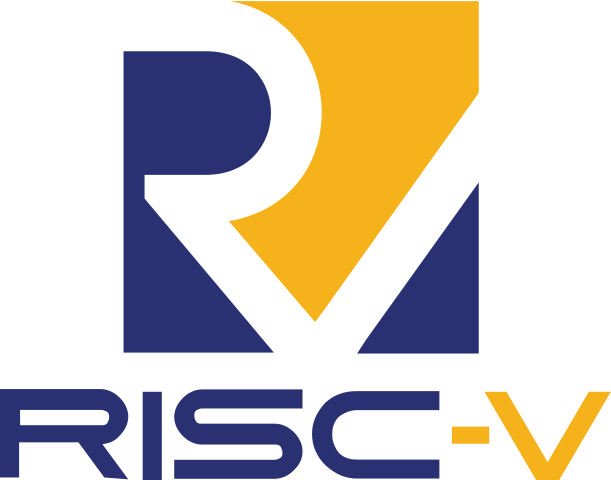
\includegraphics[width=\textwidth]{figures/RISC-V-logo-square.svg.png}
        \caption{Logo de RISC-V. Wikimedia Commons}
        \label{fig:logoRISCV}
    \end{minipage}\hfill
    \begin{minipage}{0.45\textwidth}
        \centering
        
\includegraphics[width=\textwidth]{figures/x-heep-outline.png}
        \caption{Logo de X-HEEP. Fuente: \cite{xheepLogo}}
        \label{fig:imagen2}
    \end{minipage}
    \caption{Título común para ambas figuras.}
    \label{fig:dosimagenes}
\end{figure}


Debido a la gran complejidad que supone el diseño \textit{hardware}, se han propuesto una gran cantidad de metodologías \cite{metodologiasHW} Entre las metodologías más utilizadas se encuentra el diseño a nivel de registro \ac{RTL}, que utiliza \ac{HDL}s como \ac{VHDL} o Verilog para especificar el comportamiento y la estructura del circuito de forma detallada. Esta aproximación ofrece un control total sobre la implementación, pero requiere un conocimiento profundo de la arquitectura y de las restricciones de temporización. Otra metodología relevante es la síntesis de alto nivel \ac{HLS}, que permite describir el hardware a partir de lenguajes de programación como C, C++ o SystemC, reduciendo el tiempo de desarrollo y facilitando la exploración de arquitecturas, aunque con un posible coste en optimización a grano fino. El diseño basado en \ac{IP} Cores reutilizables es también ampliamente empleado, permitiendo integrar bloques funcionales ya probados para acelerar la creación de sistemas complejos. A estos enfoques se suman metodologías híbridas que combinan RTL, HLS y IPs, junto con el uso de herramientas de verificación y simulación avanzadas, formando un flujo de trabajo iterativo que va desde el modelado funcional hasta la implementación física. Por ello, han surgido herramientas que simplifican todo el proceso con el objetivo de hacer el diseño \textit{hardware} algo sencillo y apto para un público más amplio, como diseñadores de \textit{software}. 

Desde hace tiempo, se han empleado herramientas \ac{CAD} con el objetivo de acelerar y automatizar la mayor cantidad de los procesos necesarios en el diseño \textit{hardware}. En este contexto, destacan las herramientas de la empresa Xilinx, actualmente propiedad de AMD \cite{compraXilinx}. Su plataforma principal, Vivado Design Suite \cite{vivadoInfo}, ofrece un entorno unificado que abarca desde la descripción RTL tradicional hasta el diseño a través de HLS con Vitis HLS, así como la integración de IPs mediante su IP Integrator. Este enfoque fomenta un desarrollo modular, donde se combinan bloques predefinidos con lógica personalizada, optimizando el uso de recursos del FPGA y acelerando la validación del sistema. La metodología de Xilinx también pone especial énfasis en la verificación temprana mediante simulación, análisis de temporización y estimación de consumo, permitiendo corregir problemas antes de la implementación física. En proyectos orientados a System-on-Chip (SoC), se integra además el flujo de diseño para procesadores embebidos como MicroBlaze o núcleos ARM (en FPGAs con SoC integrado), así como el soporte a arquitecturas abiertas como RISC-V. Esta filosofía de diseño, ahora reforzada por la integración con AMD, apunta a ofrecer un entorno flexible y escalable, capaz de cubrir desde prototipado rápido hasta despliegues en producción de alto rendimiento. 

Dentro del campo del diseño de \textit{hardware}, destaca el apartado de las simulaciones. Esto es así debido a que el coste de un prototipo es, por lo general, demasiado elevado como para realizar pruebas sobre una plataforma física, lo cual incurriría en un coste extra de desarrollo. Por tanto, la simulación es clave, pues permite validar el diseño antes de su implementación física, ahorrando tiempo y costos asociados a posibles errores. Mediante simuladores de ciclo preciso o de alto nivel, los desarrolladores pueden verificar el comportamiento funcional, analizar el rendimiento y detectar problemas de sincronización sin necesidad de programar repetidamente el FPGA. En proyectos como X-HEEP, es posible evaluar diferentes configuraciones del núcleo RISC-V, probar periféricos personalizados y garantizar la correcta integración del sistema completo. De este modo, se minimizan riesgos y se acelera el ciclo de desarrollo, haciendo posible que las fases de depuración y optimización se realicen con mayor precisión y menor dependencia de hardware físico. 

Precisamente en la ejecución de simulaciones, a la hora de simular un conjunto indefinido de tareas, es necesario el uso de herramientas que permitan una correcta gestión de los recursos y que simplifiquen el proceso de ejecución de cada tarea. La solución planteada actualmente a esta problemática es el uso de los conocidos como RTOS, sistemas operativos livianos que, con un conjunto reducido de librerías son capaces de gestionar un diseño de forma global, algo especialmente útil en entornos embebidos, donde los plazos de tiempo generalmente son críticos.


